\documentclass{beamer}
\usepackage[utf8]{inputenc}
\usepackage[spanish]{babel}
\usepackage{bbding}
\usetheme{Madrid}
\usecolortheme[RGB={79,79,79}]{structure}
\definecolor{darkblue}{RGB}{10,5,133}
%10,5,133
\usepackage{media9}

%Justificación de todos los blocks
\usepackage{ragged2e} 
\addtobeamertemplate{block begin}{}{\justifying}

%Cambiar tamaño de los captions
\usepackage{caption}
\captionsetup{font=scriptsize,labelfont=scriptsize}

\title{Monografía}
\subtitle{Impacto de los parámetros cosmológicos en la estructura a gran escala del universo}
\author[Camilo Andrés Rivera]{Camilo Andrés Rivera 200912840\\[7mm] Asesor: Jaime Ernesto Forero.\\[3mm]}


\begin{document}

\AtBeginSection[ ]
{
	\begin{frame}
	
		\frametitle{Tabla de contenidos}
		\tableofcontents[currentsection]
		
	\end{frame}
}

\AtBeginSubsection[ ]
{
	\begin{frame}
	
		\frametitle{Tabla de contenidos}
		\tableofcontents[currentsubsection]
		
	\end{frame}
}
\begin{frame}

	\titlepage
	
\end{frame}

\begin{frame}{Agenda}
\tableofcontents
\end{frame}

%inicia presentacion
\section{Introducción y Justificación}
%================================================%
\begin{frame}
	\begin{columns}
		\begin{column}{0.4\textwidth}
			\begin{figure}[!h]
			\begin{center}
				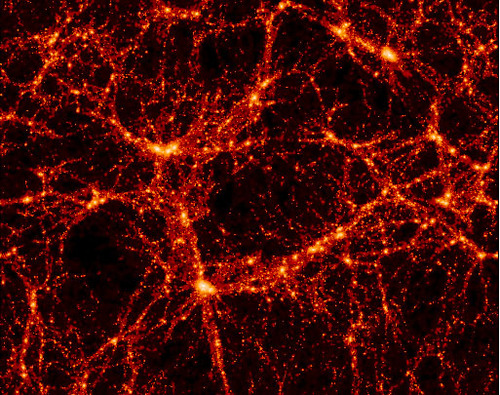
\includegraphics[width=0.9\textwidth]{im/lss.jpg}
				\caption{LSS \footnotemark[2]} 
				\label{fig:arq1}
			\end{center}
		\end{figure}
		\end{column}
		
		\begin{column}{0.4\textwidth}
			\begin{figure}[!h]
			\begin{center}
				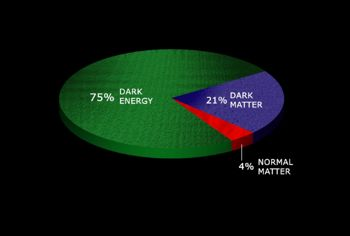
\includegraphics[width=1.1\textwidth]{im/DM.jpg}
				\caption{DM \footnotemark[3]} 
				\label{fig:arq2}
			\end{center}
		\end{figure}
		\end{column}
		\footnotetext[2]{Imagen Tomada de \cite{lss}}
		\footnotetext[3]{Imagen Tomada de \cite{dm}}
	\end{columns}
	
	\begin{block}{}
		\begin{itemize}
			\item La materia da cuenta de la estructura a gran escala del universo
			\item $\Omega_\Lambda,\Omega_{DM}, \Omega_0$
			\item A pesar de que domina la materia oscura, la energía oscura tiene un efecto sutil pero importante
		\end{itemize}
	\end{block}
\end{frame}
%================================================%
\begin{frame}{Motivación}
	 \begin{itemize}
	 	\item Anisotropías en CMB medidas por Plank
	 	\item Sensibilidad y margen de error en equipos de medición
	 	\item Detección de variaciones de al menos $5\%$
	\end{itemize}	 	
	
	\begin{block}{}
		\centering
		\LARGE{¿Cómo podemos medir los efectos de la energía oscura ($\Omega_\Lambda$)?}	
	\end{block}

\end{frame}
%================================================%
\section{Objetivos}
%================================================%
\begin{frame}{Objetivos}
	\begin{block}{General}
		Cuantificar el cambio de la estructura a gran escala del universo ante escenarios con diferentes parámetros cosmológicos.
	\end{block}
	\begin{block}{Específicos}
		\begin{itemize}
			\item Obtener una serie de universos simulados ante diferentes valores de parámetros cosmológicos.
			\item Extraer información acerca de los diferentes universos como la abundancia de halos de materia oscura y las distribuciones de velocidad entre pares de halos.
			\item Realizar un análisis comparativo entre los diferentes universos simulados
		\end{itemize}	
	\end{block}
\end{frame}
%================================================%
\section{Contexto del Proyecto}
%================================================%
\subsection{Contexto Teórico}
\begin{frame}{Evolución Universo}


\end{frame}

\subsection{Contexto Computacional}
\begin{frame}{Características de la Simulación}
	\begin{itemize}
		\item Tamaño de las simulaciones
		\begin{itemize}
			\item Cubo $\sim 500Mpc$
			\item Tiempo de evolución $\sim 13 Gyr$
			\item Número partículas $512^3$
		\end{itemize}
		\item Condiciones iniciales
		\begin{itemize}
			\item N-Genic
			\item Posiciones y velocidades
			\item $\rho$
		\end{itemize}
		\item Leyes de la física
		\item $\Omega_\Lambda$, $\Omega_0$, $H_0$
	\end{itemize}
		
\end{frame}
%================================================%
\begin{frame}{Características del Análisis}
	\begin{block}{}
	\begin{itemize}
		\item Sobredensidad
		\begin{itemize}
			\item CIC
		\end{itemize}
		\item Halos
		\begin{itemize}
			\item FoF
			\item Características de CM
			\item Identificación cruzada
			\item Diferencias y gráficas (\textit{ipython})
		\end{itemize}
	\end{itemize}
	\end{block}	
\end{frame}
%================================================%
\section{Metodología y Cronograma}
%================================================%
%\begin{frame}
%	\begin{block}{Contexto}
%	La evolución del universo y la distribución en el espacio de fase de los halos de materia ordinaria y materia oscura están fuertemente determinados por los parámetros cosmológicos $\Omega_\Lambda$, $\Omega_0$, $H_0$, entre otros.
%	La simulación de diferentes escenarios a gran escala ($\sim 1Gpc$) permite observar diferencias significativas en la estructura del universo en un análisis transversal y simultáneo.
%	\end{block}
%	\end{frame}
	%================================================%
%\begin{frame}
%	\begin{block}{Metodología}
%	\begin{itemize}
%		\item Código libre de baja dificultad de implementación (Gadget-2 \cite{gadget})
%		\item Múltiples simulaciones ($\sim 10$) variando parámetros cosmológicos
%		\item Uso del cluster de física para realizar simulaciones en paralelo en varios procesadores ($\sim 32$)
%		\item Generación de condiciones iniciales necesarias para la evolución del universo simulado		
%		\item Hacer uso de \textit{snapshots} generados por las simulaciones para realizar análisis de las estadísticas y distribuciones 
%	\end{itemize}
%	\end{block}
%\end{frame}

\begin{frame}{Metodología}
	\begin{figure}
		\centering
		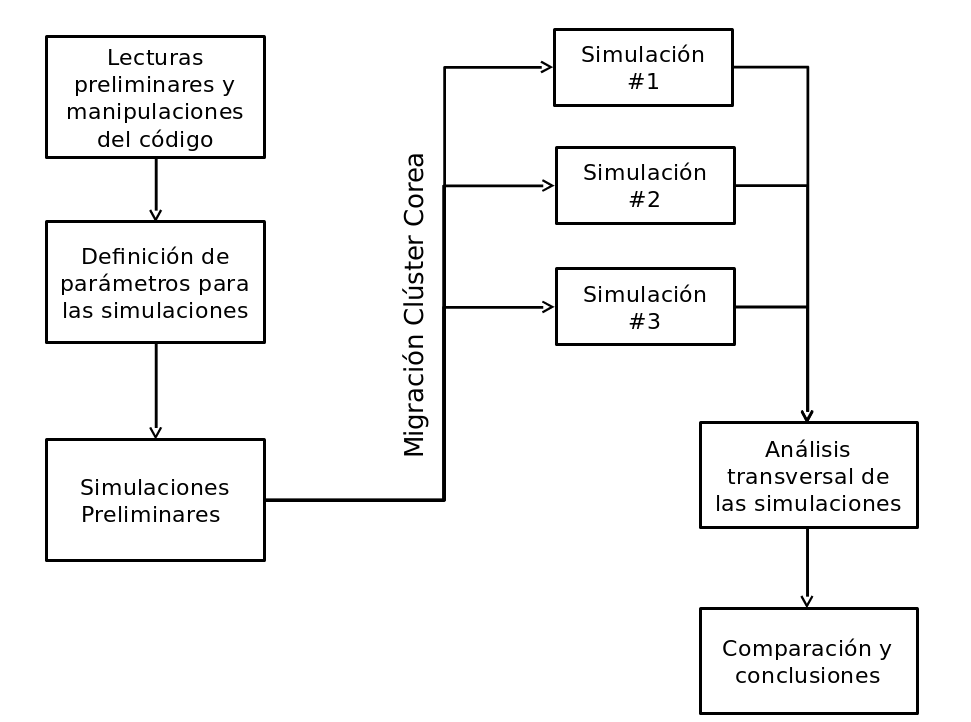
\includegraphics[width=0.7\textwidth]{im/Metodo}
		\caption{Metodología de Desarrollo}
		\label{fig:meto}
	\end{figure}

\end{frame}
%================================================%
%\subsection{Cronograma}
%================================================%
	\begin{frame}{Cronograma}
	\centering
	\begin{figure}%
		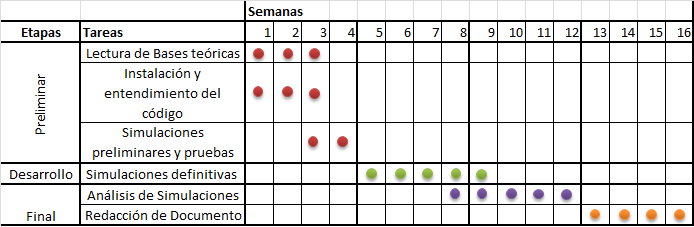
\includegraphics[width=0.9\textwidth]{im/cronograma.png}%
		\caption{Cronograma Propuesto}%
		\label{fig:crono}%
	\end{figure}
			
	\end{frame}

%================================================%
\section{Trabajo Realizado}
%================================================%
\begin{frame}{Simulaciones preliminares}
	\begin{block}{Características}
		Caja cúbica de $150 Mpc$, $128^3$ partículas, tiempo inicial de \textit{redshift} $z=63$ ($\sim 32.4 Myr$) hasta la actualidad ($\sim 13Gyr$).\\~\\
		\begin{itemize}
			\item 32 Procesadores (fiscluster)
			\item 50 snapshots
			\item $\sim 3Gb$ de almacenamiento
			\item 4 horas de simulación
			\item Variación de Sigma8 (0.9 - 0.7)
		\end{itemize}
	\end{block}	
\end{frame}

%================================================%
\begin{frame}{Simulaciones Preliminares}
	\begin{columns}
		\begin{column}{0.5\textwidth}
			\begin{figure}[!h]
			\begin{center}
				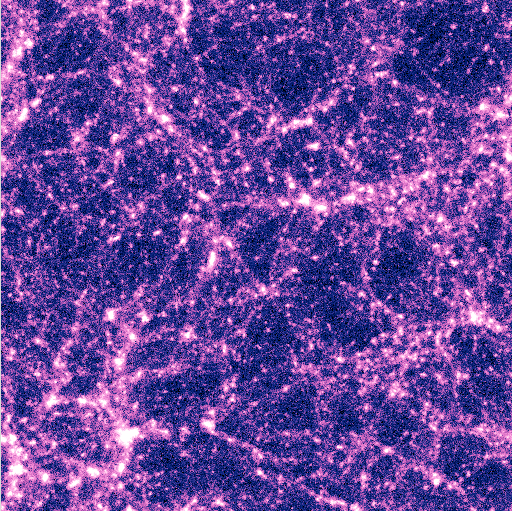
\includegraphics[width=\textwidth]{im/res1.png}
				\caption{$\sigma_8=0.9$} 
				\label{fig:res1}
			\end{center}
		\end{figure}
		\end{column}
		
		\begin{column}{0.5\textwidth}
			\begin{figure}[!h]
			\begin{center}
				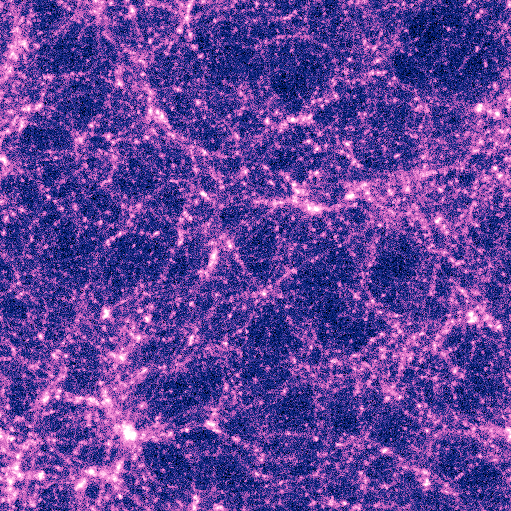
\includegraphics[width=\textwidth]{im/res2.png}
				\caption{$\sigma_8=0.7$} 
				\label{fig:res2}
			\end{center}
		\end{figure}
		\end{column}
	\end{columns}
\end{frame}

%================================================%
\begin{frame}{Simulaciones Definitivas}
	\begin{block}{Características}
		Caja cúbica de $500 Mpc$, $512^3$ partículas.\\~\\
		\begin{itemize}
			\item 32 Procesadores (KIAS)
			\item 5 snapshots
			\item $\sim 3.4Gb$ de almacenamiento por snapshot
			\item 5 días de simulación
			\item Datos de Plank
			\item Variación de $\Omega_0\pm5\%$
		\end{itemize}
	\end{block}		
	
\end{frame}
%================================================%
\subsection{Resultados}
%================================================%
\begin{frame}{Comparación de Masa}
	\begin{columns}
		\begin{column}{0.5\textwidth}
			\begin{figure}[!h]
			\begin{center}
				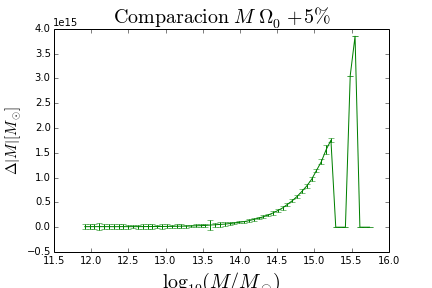
\includegraphics[width=\textwidth]{im/logm-deltam-mas}
				%\caption{$\sigma_8=0.9$} 
				\label{fig:m1}
			\end{center}
		\end{figure}
		\end{column}
		
		\begin{column}{0.5\textwidth}
			\begin{figure}[!h]
			\begin{center}
				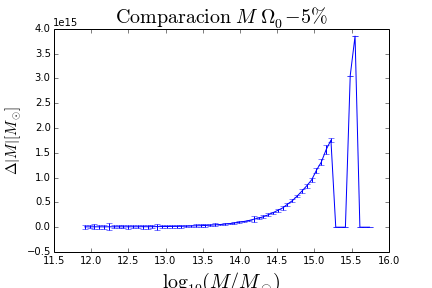
\includegraphics[width=\textwidth]{im/logm-deltam-menos}
				%\caption{$\sigma_8=0.7$} 
				\label{fig:m2}
			\end{center}
		\end{figure}
		\end{column}
	\end{columns}
\end{frame}
%================================================%
\begin{frame}{Comparación de Posición}
	\begin{columns}
		\begin{column}{0.5\textwidth}
			\begin{figure}[!h]
			\begin{center}
				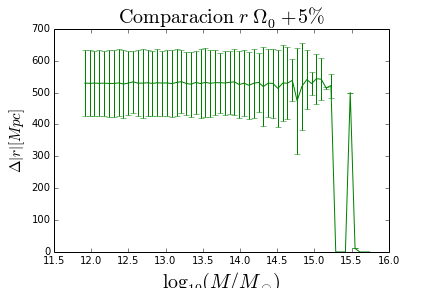
\includegraphics[width=\textwidth]{im/logm-deltap-mas}
				%\caption{$\sigma_8=0.9$} 
				\label{fig:p1}
			\end{center}
		\end{figure}
		\end{column}
		
		\begin{column}{0.5\textwidth}
			\begin{figure}[!h]
			\begin{center}
				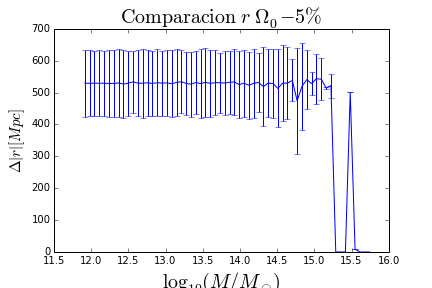
\includegraphics[width=\textwidth]{im/logm-deltap-menos}
				%\caption{$\sigma_8=0.7$} 
				\label{fig:p2}
			\end{center}
		\end{figure}
		\end{column}
	\end{columns}
\end{frame}
%================================================%
\begin{frame}{Comparación de Velocidad}
	\begin{columns}
		\begin{column}{0.5\textwidth}
			\begin{figure}[!h]
			\begin{center}
				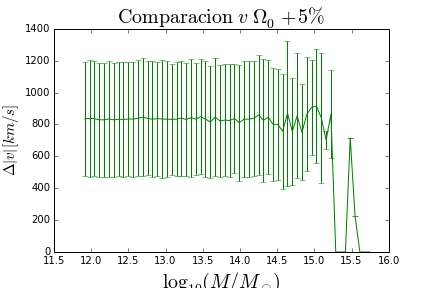
\includegraphics[width=\textwidth]{im/logm-deltav-mas}
				%\caption{$\sigma_8=0.9$} 
				\label{fig:v1}
			\end{center}
		\end{figure}
		\end{column}
		
		\begin{column}{0.5\textwidth}
			\begin{figure}[!h]
			\begin{center}
				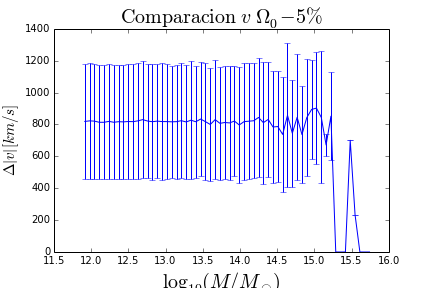
\includegraphics[width=\textwidth]{im/logm-deltav-menos}
				%\caption{$\sigma_8=0.7$} 
				\label{fig:v2}
			\end{center}
		\end{figure}
		\end{column}
	\end{columns}
\end{frame}
%================================================%
\begin{frame}{Distribuciones de cambios de velocidad y masa}
	\begin{columns}
		\begin{column}{0.5\textwidth}
			\begin{figure}[!h]
			\begin{center}
				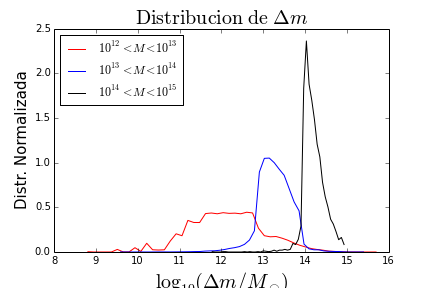
\includegraphics[width=\textwidth]{im/deltammas}
				%\caption{$\sigma_8=0.9$} 
				\label{fig:mm1}
			\end{center}
		\end{figure}
		\end{column}
		
		\begin{column}{0.5\textwidth}
			\begin{figure}[!h]
			\begin{center}
				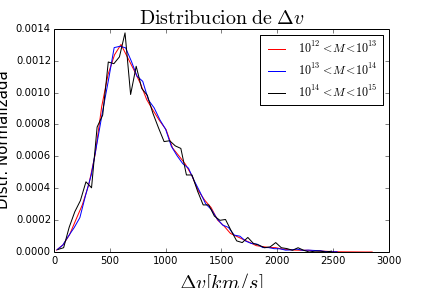
\includegraphics[width=\textwidth]{im/deltavmas}
				%\caption{$\sigma_8=0.7$} 
				\label{fig:vv1}
			\end{center}
		\end{figure}
		\end{column}
	\end{columns}
\end{frame}
%================================================%
\section{Conclusiones}
%================================================%
	\begin{frame}
		\begin{center}
			\textcolor{darkblue}{\Huge{MUCHAS GRACIAS}}
		\end{center}
		
	\end{frame}
%================================================%
	\begin{frame}[allowframebreaks]{Referencias}
		\begin{thebibliography}{}
			\bibitem{gadget} V. Springel. The cosmological simulation code gadget-2. Monthly Notices of the Royal Astronomical Society, 364, 2005.
			\bibitem{dm} Conservapedia. Dark Matter. [En línea] Disponible en: \url{http://www.conservapedia.com/images/thumb/4/44/DarkMatterNASA1.jpg/350px-DarkMatterNASA1.jpg}
			\bibitem{lss} Smithsonian Astrophysical Observatory. The Cosmic Infrared Background. [En línea] Disponible en:\url{http://www.cfa.harvard.edu/sites/www.cfa.harvard.edu/files/images/news//su201231.jpg}	
			\bibitem{hed} HETDEX - Hobby-Eberly Telescope Dark Energy Experiment \url{http://hetdex.org/}
			\bibitem{loeb} A. Loeb. How did the first stars and galaxies form? Princeton University Press, Princeton, NJ,
2010. 3, 4, 7

			
	\end{thebibliography}
%	\bibliographystyle{abbrv}
%	\bibliography{references}
	\end{frame}
%================================================%
\end{document}
